\documentclass[11pt]{article}
\usepackage[scaled=0.92]{helvet}
\usepackage{geometry}
\geometry{letterpaper,tmargin=1in,bmargin=1in,lmargin=1in,rmargin=1in}
\usepackage[parfill]{parskip} % Activate to begin paragraphs with an empty line rather than an indent %\usepackage{graphicx}
\usepackage{amsmath,amssymb, mathrsfs, dsfont, stackrel}
\usepackage{tabularx}
\usepackage[font=footnotesize,labelfont=bf]{caption}
\usepackage{graphicx}
\usepackage{xcolor}
%\usepackage[linkbordercolor ={1 1 1} ]{hyperref}
%\usepackage[sf]{titlesec}
\usepackage{natbib}
\usepackage{../../Tianpei_Report}
%\usepackage{appendix}
%\usepackage{algorithm}
%\usepackage{algorithmic}

%\renewcommand{\algorithmicrequire}{\textbf{Input:}}
%\renewcommand{\algorithmicensure}{\textbf{Output:}}



\begin{document}
\title{Lecture 1: Basics of Monte Carlo Methods}
\author{ Tianpei Xie}
\date{Sep. 28th., 2022 }
\maketitle
\tableofcontents
\newpage
\allowdisplaybreaks
\section{Basic Concepts}
\subsection{Random variable generation}
\begin{itemize}
\item The most fundamental methods for random variable generation is the \emph{\textbf{uniform pseudo-random number generator}}.
\begin{definition}
 A \emph{uniform pseudo-random number generator} is an algorithm which, starting from an initial value $u_0$ and a transformation $D$, produces a sequence $(u_i) = (D^i(u_{0}))$ of values in $[0, 1]$. For all $n$, the values $(u_1, \ldots , u_n)$ reproduce the behavior of an \emph{iid} sample $(V_1, \ldots, V_n)$ of uniform random variables when compared through a usual set of tests.
 \end{definition}

\item This definition is clearly restricted to testable aspects of the random variable generation, which are connected through the deterministic transformation $u_i = D^{i}(u_{i-1})$. Thus, the validity of the algorithm consists in the verification that the sequence $U_1, \ldots, U_n$ leads to acceptance of the hypothesis
\begin{align*}
H_0: \quad U_1, \ldots, U_n \;\text{ i.i.d. } \cU[0,1]
\end{align*}

\item Definition above is therefore \emph{\textbf{functional}}: An algorithm that generates uniform numbers is acceptable if it is not rejected by a set of tests. 

\item This methodology is not without problems, however. Consider, for example, particular applications that might demand a large number of iterations, as the theory of large deviations, or particle physics, where algorithms resistant to standard tests may exhibit fatal faults. In particular, algorithms having hid- den periodicities (e.g. Ising models) or which are not uniform for the smaller digits may be difficult to detect.

\item Given uniform distribution $\cU[0,1]$, and a known c.d.f. $F(x)$, we can generate samples via the \emph{\textbf{inverse transform}} method. \citep{robert1999monte}

\begin{definition}
For a \textbf{\emph{non-decreasing}} function $F$ on $\bR$, the \underline{\emph{\textbf{generalized inverse}}} of $F$, $F^{-}$, is the function defined by
\begin{align}
F^{-}(u) &= \inf\{x \in \cR(F): F(x) \ge u \}. \label{eqn: quantile_function}
\end{align} where $\cR(F)$ is the range of $F$. If $F$ is the cumulative distribution function $F_{X}(x) = P(X \le x)$, then $F_{X}^{-1}$ is called \underline{\textbf{\emph{quantile function}}}.
\end{definition}

\item We then have the following lemma, sometimes known as the \textbf{probability integral transform}, which gives us a representation of any random variable as a transform of a uniform random variable.
\begin{lemma} \citep{robert1999monte}\\
If $U \sim \cU[0,1]$, then the random variable $F^{-}(U)$ has the distribution $F$.
\end{lemma}

\item Examples for some quantile functions \citep{robert1999monte}
\begin{itemize}
\item \textbf{Exponential distribution}: $F^{-}(u) = -\log(1-u)$. Since $U$ and $1-U$ are both uniform in $[0,1]$, $X = \log(U)\sim \exp(1)$ is exponential distributed with $\lambda = 1$;
\item \textbf{Gamma distribution} and $\chi^2$ distribution can be generated from the exponential distribution $\exp(1)$
\begin{align*}
Y &= \beta\,\sum_{j=1}^{a}X_j \sim \Gamma(a, \beta),; a\in \bN_{}+ \\
Y &= 2 \sum_{j=1}^{\nu} X_j \sim \chi^2_{2\nu} ; \nu\in \bN_{}+
\end{align*}
\item \textbf{Normal distribution}:
\begin{align*}
X_1 &= \sqrt{-2\log(U_1)}\cos(2\pi U_2)\\
X_2 &= \sqrt{-2\log(U_1)}\sin(2\pi U_2)
\end{align*} where $U_1, U_2$ are i.i.d from $\cU[0,1]$. Then $X_1, X_2$ are i.i.d from $\cN(0,1)$.
\end{itemize}

\item Theoretically, any random variable can be generated using the inverse transform. But in practice, it is only available when we can compute the c.d.f and its inverse $F^{-}$ explicitly. 
\end{itemize}

\subsection{Why Monte Carlo ?}
\begin{itemize}
\item The most fundamental operations in probabilistic modeling and statistics involve \underline{\emph{\textbf{integration}}} on \underline{\textbf{high dimensional spaces}}:
\begin{align*}
I := \int_{\cX} g(\mb{x})d\mb{x}
\end{align*} For example, 
\begin{itemize}
\item \underline{\emph{\textbf{Expectation}}}: 
\begin{align}
\E{\mb{X}\sim p}{h(\mb{X})} &= \int_{\cX}h(\mb{x})p(\mb{x}) d\mb{x}  \label{eqn: exp_integration}
\end{align} where $\mb{x}:= [x_1,\ldots, x_d]$

\item \underline{\emph{\textbf{Marginalization}}}:
\begin{align*}
P(x_1,\ldots, x_{i-1}, x_{i+1} \ldots, x_d) &= \int_{x_i \in \cX_i}P(x_1,\ldots, x_{i-1}, x_i, x_{i+1} \ldots, x_d) d x_i
\end{align*}

\item \underline{\emph{\textbf{Conditioning}}}:
\begin{align*}
P(x_1,\ldots, x_{i-1}, x_{i+1} \ldots, x_d \,|\, X_i = x_i) 
&= \frac{P(x_1,\ldots, x_{i-1}, x_i, x_{i+1} \ldots, x_d)}{ \int_{\mb{x}_{-i} \in \mb{X}_{-i}}P(x_1,\ldots, x_{i-1}, x_i, x_{i+1} \ldots, x_d) d\mb{x}_{-i}}
\end{align*} where $\mb{x}_{-i} = [x_1,\ldots, x_{i-1}, x_{i+1} \ldots, x_d]$.
\end{itemize}

\item This is especially important for \emph{\textbf{Bayesian inference}} and analysis. Since it replies on computing \emph{posterior distribution}  given data using \textbf{the Bayes rule}
\begin{align*}
P(\mb{\Theta} | \cD) &= \frac{P(\cD | \mb{\Theta}) P(\mb{\Theta})}{P(\cD)}\\
 &= \frac{P(\cD | \mb{\Theta}) P(\mb{\Theta})}{\int_{\mb{\Theta}} P(\cD | \mb{\Theta}) P(\mb{\Theta}) d \mb{\Theta}}\\
 \Rightarrow \log P(\mb{\Theta} | \cD)  &= \log P(\cD | \mb{\Theta}) + \log P(\mb{\Theta}) - \log \int_{\mb{\Theta}} P(\cD | \mb{\Theta}) P(\mb{\Theta}) d \mb{\Theta}
\end{align*} where $\cD: =\set{\mb{X}_1, \ldots, \mb{X}_n}$ are i.i.d. samples and $\mb{\Theta}$ is a set of parameters for model $p(\cD | \mb{\Theta})$.

\item The main challenge for Bayesian methods in high dimensional space is to compute the normalization factor
\begin{align*}
\int_{\mb{\Theta}} P(\cD | \mb{\Theta}) P(\mb{\Theta}) d \mb{\Theta}.
\end{align*}

\item The \textbf{\emph{log-partition function}} in \textbf{exponential families} play a critical role since it defines a \emph{bijective mapping} from \emph{natural parameters} to \emph{mean parameters} and is related to \textbf{negative entropy} via \emph{variational principles}. The log-partition function for exponential families is a convex function as well.
\begin{align*}
A(\mb{\eta}) &= \log \int_{\Omega}\exp\paren{\inn{\mb{\eta}}{\mb{\phi}(\mb{x})}}d\mb{x}
\end{align*}

\item It is natural to propose using a sample $(\mb{X}_1, \ldots , \mb{X}_m)$ generated from the density $p$ to \emph{approximate integration} by the \emph{empirical average}. This approach is referred to as the \emph{\textbf{Monte Carlo methods}}. Specifically from \eqref{eqn: exp_integration}, 
\begin{align}
\overline{h}_{m} &= \frac{1}{m}\sum_{i=1}^{m}h(\mb{X}_{i}) \label{eqn: exp_integration_monte_carlo}.
\end{align} since $\overline{h}_{m}$ converges almost surely to $\E{\mb{X}\sim p}{h(\mb{X})}$ by the \emph{Strong Law of Large Numbers}. Moreover, when $\overline{h}_{m}$ has a finite expectation under $p$, the speed of convergence of $\overline{h}_{m}$ can be assessed since the variance 
\begin{align*}
\text{Var}\paren{\overline{h}_{m}} &= \frac{1}{m}\int_{\cX}\paren{h(\mb{x}) - \E{\mb{X}\sim p}{h(\mb{X})}}^{2}p(\mb{x}) d\mb{x}
\end{align*} can also be estimated from the sample $(\mb{X}_1, \ldots , \mb{X}_m)$ through
\begin{align*}
v_{m} &= \frac{1}{m}\sum_{i=1}^{m}\paren{h(\mb{X}_{i}) - \overline{h}_{m}}^2
\end{align*}
For $m$ large,
\begin{align*}
\frac{h(\mb{X}) - \overline{h}_{m}}{\sqrt{v_{m}}} \rightarrow \cN(0, 1).
\end{align*} This leads to the construction of a \emph{\textbf{convergence test}} and of \emph{\textbf{confidence bounds}} on the approximation of $\E{\mb{X}\sim p}{h(\mb{X})}$.

\end{itemize}

\section{Rejection and Weighting}
\subsection{Reject Sampling}
\begin{itemize}
\item There exists a fundamental idea underlying the \emph{\textbf{Accept-Reject sampling method}}:
\begin{theorem} (\textbf{Fundamental Theorem of Simulation}) \citep{robert1999monte}\\
Simulating $X \sim F(x)$ is equivalent to simulating
\begin{align*}
(X,U) \sim \cU\{(x,u): 0 < u < F(x)\}.
\end{align*}
\end{theorem} 

In essence, If $f$ is the density of interest, on an arbitrary space, we can write this theorem as 
\begin{align*}
f(x) &= \int_{0}^{f(x)} d u.
\end{align*} Thus, $f$ appears as the marginal density (in $X$) of the joint distribution, $(X,U) \sim \cU\{(x,u): 0 < u < f(x)\}$.

\item  Suppose $l(\mb{x}) = c\,f(\mb{x})$ is computable, where $f$ is the probability density and $c$ is unknown. If we can find a sampling distribution $g(\mb{x})$ and a \emph{\textbf{covering constant}} $M$ so that $M g(\mb{x}) \ge l(\mb{x})$ (i.e. the envelop property) is satisfied for all $\mb{x}$. We can apply the following procedure:

\emph{\textbf{Accept-Reject sampling sampling}} \citep{liu2001monte}
\begin{enumerate}
\item Draw sample $\mb{x}$ from $g(\,)$ and compute the \textbf{ratio}
\begin{align*}
r &= \frac{l(\mb{x})}{M\,g(\mb{x})}\quad (\le 1)
\end{align*}
\item Flip a coin with \textbf{success probability} $r$. If the head turns up, accept $\mb{x}$; otherwise, reject $\mb{x}$
\end{enumerate} 
Then the accepted samples follow the distribution $f(\mb{x})$.
\begin{proof}
Let $I\in \set{0, 1}$ be the event when head turns up ($=1$) vs. tail turns up ($=0$). 
\begin{align*}
P(I=1) &= \int P(I=1 | \mb{x}) g(\mb{x}) d\mb{x} = \int \frac{c\, f(\mb{x})}{M\,g(\mb{x})}g(\mb{x}) d\mb{x} = \frac{c}{M}
\end{align*}
Then 
\begin{align*}
P(\mb{x} | I=1) &= \frac{g(\mb{x}) \frac{c\, f(\mb{x})}{M\,g(\mb{x})} }{P(I=1)} = f(\mb{x}). \qed
\end{align*}
\end{proof}

\item This is equivalent to say 
\begin{enumerate}
\item Draw sample $\mb{X}$ from $g(\mb{x})$ and $U$ from $\cU[0,1]$

\item Accept $\mb{Y} = \mb{X}$ if $U\le f(\mb{x})/(M\,g(\mb{x}))$; 

\item Otherwise, return to step 1.
\end{enumerate}

\item The key for a successful application of rejection sampling method is to choose a good trial distribution $g(\cdot)$ so that $M$ is \textbf{small}. In high dimensional settings, it is usually hard to find a good trial distribution.

\item \begin{lemma}
If there exist a density $g_{m}(\mb{x})$, a function $g_{l}(\mb{x})$ and a constant $M$ such that
\begin{align*}
g_l(\mb{x}) \le f(\mb{x}) \le M\,g_{m}(\mb{x}) 
\end{align*}
then the algorithm \emph{\textbf{Envelope Accept-Reject}}
\begin{enumerate}
\item Draw sample $\mb{X}$ from $g_{m}(\mb{x})$ and $U$ from $\cU[0,1]$

\item Accept $\mb{X}$ if $U\le g_{l}(\mb{x})/(M\,g_{m}(\mb{x}))$; 

\item Otherwise, accept $\mb{X}$ if $U\le f(\mb{x})/(M\,g_{m}(\mb{x}))$ else return to step 1.
\end{enumerate}
produces random variables that are distributed according to $f$.
\end{lemma}

\item By the construction of a lower envelope on $f$, based on the function $g_{l}$, the number of evaluations of $f$ is potentially decreased by a factor
\begin{align*}
\frac{1}{M}\int g_l(\mb{x}) d\mb{x},
\end{align*}
which is the probability that $f$ is not evaluated. This method is called the \emph{\textbf{squeeze principle}}.


\begin{figure}
\begin{minipage}[t]{1\linewidth}
  \centering
  \centerline{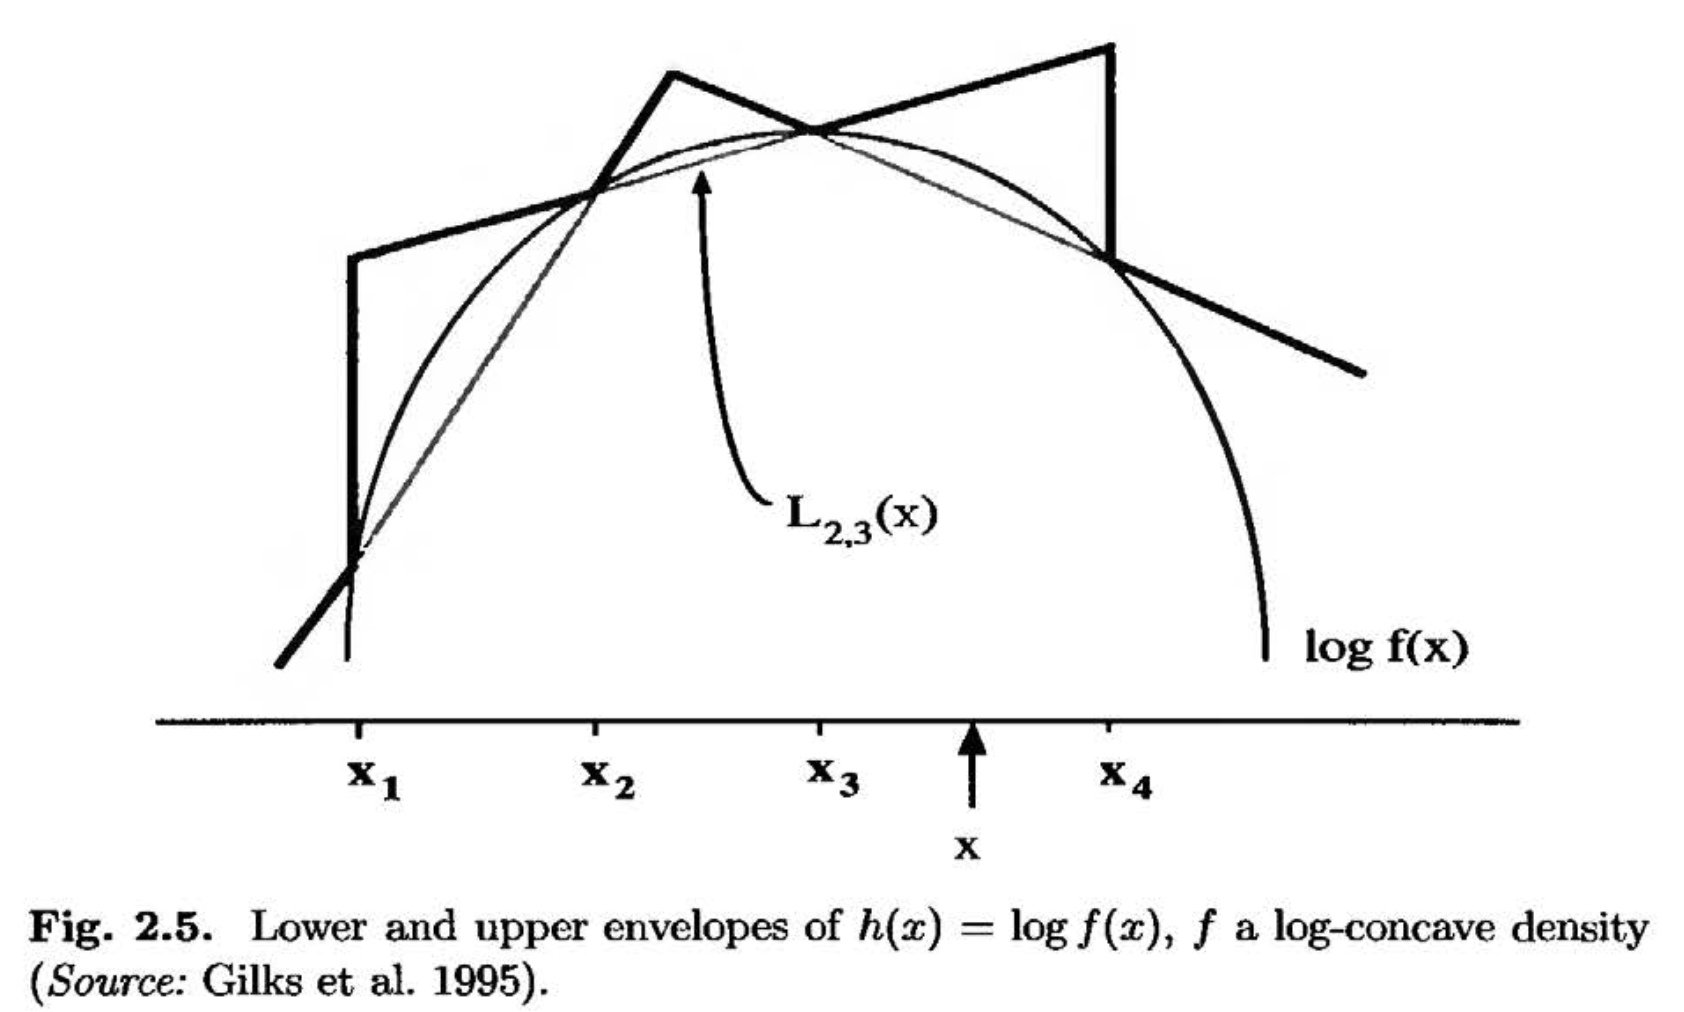
\includegraphics[scale = 0.45]{reject_ars.png}}
\end{minipage}
\caption{\footnotesize{\textbf{The log-concave function $h$ and its upper and lower bounds \citep{robert1999monte}}}}
\label{fig: simpson_paradox}
\end{figure}


\item For the exponential families, the density function
\begin{align*}
f(\mb{x}; \mb{\theta}) &= h(\mb{x})\exp\paren{\inn{\mb{\theta}}{\mb{x}} - A(\mb{\theta})}
\end{align*} is \emph{log-concave} in terms of $\mb{x}$.  An envelop accept-reject sampling method is discussed in \citep{robert1999monte}. The method is called \underline{\emph{\textbf{adaptive rejection sampling (ARS)}}} and it provides a sequential evaluation of lower and upper envelopes of the density $f$ when $h = \log f$ is concave. Consider a set of $n$ samples $\cD_{n} = \set{\mb{x}_i}$. For each sample $\mb{x}_i$, $h(\mb{x}_i) = \log f(\mb{x}_i)$ is concave, so the following upper bound and lower bound can be found using linear segments $L_{i,i+1}$ through $(\mb{x}_i, h(\mb{x}_i))$ and $(\mb{x}_{i+1}, h(\mb{x}_{i+1}))$. Define
\begin{align*}
\overline{h}_{n}(\mb{x}) &:= \min\set{L_{i-1,i}(\mb{x}), L_{i+1,i+2}(\mb{x})};\\
\underline{h}_{n}(\mb{x}) &:= L_{i,i+1}(\mb{x}).
\end{align*} Then by concavity of $h$, for $\mb{x} \in [\mb{x}_{i}, \mb{x}_{i+1}]$
\begin{align*}
\underline{h}_{n}(\mb{x})  \le h(\mb{x}) \le \overline{h}_{n}(\mb{x})
\end{align*} Therefore, for $\underline{f}_n(\mb{x}) = \exp \underline{h}_n(\mb{x})$ and $\overline{f}_n(\mb{x}) = \exp \overline{h}_n(\mb{x})$ implies that
\begin{align*}
\underline{f}_n(\mb{x}) \le f(\mb{x}) \le \overline{f}_n(\mb{x}) = \omega_{n}\,g_{n}(\mb{x}) 
\end{align*} where $\omega_{n}$ is a normalization factor so that $g_{n}(\mb{x})$ is a density. 

Then the \underline{\emph{\textbf{adaptive rejection sampling (ARS)}}} is 
\begin{enumerate}
\item Initiate $\cD_{n} = \set{\mb{X}_1, \ldots, \mb{X}_{n}}$. Compute the line segments $L_{i,i+1}$, $i=0,\ldots, n-1$.

\item Draw sample $\mb{X}$ from $g_{n}(\mb{x})$ and $U$ from $\cU[0,1]$

\item Accept $\mb{X}$ if $U\le \underline{f}_n(\mb{x})/(\omega_{n}\,g_{n}(\mb{x}))$;
\item Otherwise, accept $\mb{X}_{n}  = \mb{X}$ if $U\le f(\mb{x})/(\omega_{n}\,g_{n}(\mb{x}))$
      and update $\cD_{n+1} = \cD_{n} \cup \set{\mb{X}_{n}}$.
\end{enumerate}

An interesting feature of this algorithm is that the set $\cD_{n}$ is only updated when $f(\mb{x})$ has been previously computed. As the algorithm produces variables the lower bound $\underline{f}_n(\mb{x})$ and upper bound $\overline{f}_n(\mb{x})$ become increasingly accurate and, therefore, we progressively reduce the number of evaluations of $f$.
\end{itemize}

\subsection{Variance Reduction}
We introduce several techniques that reduce variance while maintain the unbiasness of estimator.
\begin{itemize}
\item \textbf{Stratified sampling}: We partition the region $\cX$ into $k$ sub-regions $\cX^{i}$ and suppose that the probability distribution $f$ in each sub-regions is \emph{\textbf{relative homogeneous}}. Then we can generate samples $\mb{X}_{1}^{i}, \ldots, \mb{X}_{m_i}^{i}$ from each region $\cX^{i}$ and compute the region-wise sample average 
\begin{align*}
\bar{\mu}_{m_i}^{i} &= \frac{1}{m_i}\sum_{j=1}^{m_i}f(\mb{X}_{j}^{i})
\end{align*} Then the final result is the average of region-wise sample average $\bar{\mu} = \sum_{i=1}^{k}\bar{\mu}_{m_i}^{i}$ and the variance $\bar{\sigma}^2 = \sum_{i=1}^{k}\frac{\sigma_{i}^{2}}{m_i}$, which is reduced from original. 

Clearly, if the probability distribution is not homogeneous within each region, the stratified sampling would increase the bias and makes the estimate less accurate.

\item \underline{\textbf{Rao-Blackwellization}}: An approach to reduce the variance of an estimator is to use the \emph{conditioning inequality}
\begin{align}
\text{var}(\E{}{\delta(\mb{X})|\mb{Z}}) &\le \text{var}(\E{}{\delta(\mb{X})}) \label{eqn: rao_blackwell}
\end{align} sometimes called \textbf{\emph{Rao-Blackwellization}} \citep{liu2001monte} because the inequality is associated with the \emph{Rao-Blackwell Theorem} \citep{lehmann2006theory}, although the conditioning is not always in terms of sufficient statistics. This method reflects a \textbf{basic principle}: \emph{\textbf{one should carry out analytical computation as much as possible}}. The more information available for sampler, the less variance it would have. 

Suppose the sample can be decomposed into two parts $(\mb{X}, \mb{Z})$ and the conditional expectation can be carried out explicitly $\E{}{h(\mb{X}) | \mb{Z}}$ for each sub-population $(\mb{X}, \mb{Z}_i)$, then the estimator 
\begin{align*}
\hat{I}_{m} &= \frac{1}{m}\sum_{i=1}^{m}\E{}{h(\mb{X}) | \mb{Z}_{i}}
\end{align*} is unbias and has lower variance than the direct sample average of $h(\mb{X}_{j})$. In statistic, $\hat{I}_{m}$ is often called \emph{\textbf{mixture estimator}} since it combine a mixture of distributions for each sub-population.

\item \textbf{Control Variates Methods}: In this method, one uses a \emph{\textbf{control variate}} $C$ that is highly correlated with sample $\mb{X}$ to reduce the variance. Suppose that $\mu_{C} = \E{}{C}$ is known and the sample estimator
\begin{align*}
h(X):= X(b) &= X + b\paren{C - \mu_{C}},
\end{align*} which has the same mean as $\mb{X}$. Suppose that the optimal weight $b^{*} = \text{Cov}(X\,C)/\text{var}(C)$ can be computed explicitly, the variance of $\mb{X}(b)$
\begin{align*}
\text{var}(X(b)) &= \text{var}(X) - 2\,b\,\text{Cov}(X\,C) +  b^2 \,\text{var}(C)\\
&= (1- \rho_{X,C}^2)\;\text{var}(X) \le \text{var}(X).
\end{align*}

Note that the technique of control variates is manageable only in very specific cases: the control function $\mu_{C} = \E{}{C}$ must be available, as well as the optimal weight $b^{*}$.

\item \textbf{Antithetic Variates Methods}: This method describes a way of \textbf{creating negative correlated samples}. Suppose $X_1 = F^{-1}(U)$ for some random variable $U \sim \cU[0,1]$. Note that $X_2 = F^{-1}(1- U)$ follows the same distribution as $X_1$. $X_2$ is called \textbf{\emph{antithetic variables}}. More generally, let $g$ be a monotone function on $[0,1]$, so that for any $u_1, u_2 \in [0,1]$
\begin{align*}
(g(u_1) - g(u_2))\,(g(1-u_1) - g(1- u_2)) \le 0. 
\end{align*} Then for two i.i.d random variables $U_1, U_2 \sim \cU[0,1]$, $X_1 = g(U)$ and $X_2 = g(1- U)$ we have
\begin{align*}
\E{}{(g(U_1) - g(U_2))\,(g(1-U_1) - g(1- U_2))} &= \text{Cov}(X_1\, X_2) \le 0
\end{align*} Thus the variance of $\frac{1}{2}(X_1 + X_2)$ is less than the variance of two independent samples from Monte Carlo simulator. 
\end{itemize}

\subsection{Importance Sampling}
\begin{itemize}
\item The vanilla rejection sampling method suffers from \emph{\textbf{low sample efficiency and slow convergence}} since it wasted a lot effort evaluating random samples located in regions where the target function value $h(\mb{x})p(\mb{x})$ is almost zero. 

\item The \emph{\textbf{importance sampling}} idea suggests that one should \textbf{focus on regions of "importance"} so as to save computational resources. It is important to note that in high dimensional space, the support of the target distribution is exponentially small as compared to the entire region $\cX$. In high dimensional setting, the \textbf{vanilla Monte Carlo methods are bound to fail}.

\item Consider the expectation estimation
\begin{align}
\mu = \E{\mb{X}\sim p}{h(\mb{X})} &= \int_{\cX}h(\mb{x})p(\mb{x}) d\mb{x} \nonumber\\
&=\E{\mb{X}\sim g}{\frac{p(\mb{X})}{g(\mb{X})}h(\mb{X})} := \E{\mb{X}\sim g}{w(\mb{X})h(\mb{X})} \label{eqn: importance_sampling}\\
&= \int_{\cX} w(\mb{x})h(\mb{x})g(\mb{x}) d\mb{x} \nonumber\\
\text{where }w(\mb{x}) &:= \frac{p(\mb{x})}{g(\mb{x})} \text{ is the \emph{\textbf{importance weight.}}} \nonumber
\end{align}

\item The \underline{\emph{\textbf{Importance Sampling Algorithm}}} \citep{liu2001monte, robert1999monte} is as below:
\begin{enumerate}
\item Draw $\mb{X}_1, \ldots, \mb{X}_{m} \sim g(\mb{x})$ where $g$ is trial distribution;
\item Calculate \emph{the importance weight} $w(\mb{x})$: 
\begin{align*}
w_i := w(\mb{X}_i) &= \frac{p(\mb{X}_i)}{g(\mb{X}_i)}, \quad i=1,\ldots, m
\end{align*}
\item Approximate $\mu$ by 
\begin{align}
\hat{\mu} &= \frac{\sum_{i=1}^{m}w_i\,h(\mb{X}_i)}{\sum_{i=1}^{m}w_i} \label{eqn: importance_sampling_estimate}
\end{align}
Another way to approximate $\mu$ is via the unbiased estimator
\begin{align}
\hat{\mu} &= \frac{1}{m}\sum_{i=1}^{m}w_i\,h(\mb{X}_i) \label{eqn: importance_sampling_estimate2}
\end{align}
\end{enumerate} The normalized estimator \eqref{eqn: importance_sampling_estimate} is \textbf{\emph{biased}} but as $m\rightarrow \infty$ $\hat{\mu}\rightarrow \mu$, i.e. it is \emph{\textbf{asymptotically} unbiased}.

\item While the \eqref{eqn: importance_sampling_estimate2} converges to $\E{p}{h}$ almost surely, its variance 
\begin{align}
\E{g}{\frac{p^2(\mb{X})}{g^2(\mb{X})}h^2(\mb{X})} = \E{p}{\frac{p(\mb{X})}{g(\mb{X})}h^2(\mb{X})} = \int_{\cX} \frac{p^2(\mb{x})}{g(\mb{x})}h^2(\mb{x}) d\mb{x} < \infty \label{eqn: importance_sampling_variance}
\end{align} need to be finite. Thus $\text{supp}(g) \supset \text{supp}(p)$. In practice, the importance sampling works \textbf{poorly} (high-amplitude \textbf{\emph{jumps}}, \emph{\textbf{instability}} of the path of the average, \emph{\textbf{slow convergence}}) when 
\begin{align*}
\int_{\cX}\frac{p^2(\mb{x})}{g(\mb{x})} d\mb{x} = \infty.
\end{align*} A "\emph{Rule of thumb}" estimate of the variance is $\text{var}(\hat{\mu}) \approx \text{var}_{g}(h)\,\E{g}{w^2}$. Geweke (1989) mentions two types of \emph{sufficient conditions} for finite variance estimator:
\begin{enumerate}
\item $p(\mb{x})/g(\mb{x}) < M,\; \forall \mb{x}\in \cX$ and $\text{var}(h) < \infty$;
\item $\cX$ is compact, $p(\mb{x}) < F$ and $g(\mb{x}) > \epsilon, \;\forall \mb{x} \in \cX$.
\end{enumerate} Note that the first condition implies that the rejection sampling also applies.

On the other hand, \eqref{eqn: importance_sampling_estimate} can achieve finite variance and converges to $\E{p}{h}$ when $m\rightarrow \infty$. 

\item The \emph{\textbf{relative efficiency}} is defined as ratio between variance of vanilla Monte Carlo sampler and importance sampler: 
\begin{align*}
\text{RE} &= \frac{\frac{1}{m}\sum_{i=1}^{m}h(\mb{Y}_i)}{\frac{1}{m}\sum_{i=1}^{m}w_i\,h(\mb{X}_i)} \rightarrow 1,
\end{align*} if $w_i \rightarrow 1, \forall\,i$ or $\text{var}_{g}(w)\rightarrow 0$. Note that $\E{g}{w} = \E{g}{\frac{p}{g}} = 1$. Therefore $\text{RE} \le 1$. This is the price we pay for sampling via simpler instrumental distribution $g$.
If we use the normalized weight estimator \eqref{eqn: importance_sampling_estimate}, the relative efficiency is about
\begin{align}
\text{RE} &\approx \frac{1}{1 + \text{var}_{g}(w)} \label{eqn: importance_sampling_rel_eff}
\end{align} The \emph{\textbf{effective sample size (ESS)}} is thus 
\begin{align*}
\text{ESS} & \approx \frac{m}{1 + \text{var}_{g}(w)}.
\end{align*} These approximations do not involve $h$. Here we assume that 
\begin{align*}
\E{p}{(w(\mb{X}) - \E{p}{w(\mb{X})})(h(\mb{X}) - \mu)} \text{ is small}.
\end{align*}

\item For optimal choice of $g$ in \eqref{eqn: importance_sampling_estimate2}, we have the following theorem
\begin{theorem} \citep{robert1999monte}
The choice of g that minimizes the variance of the estimator \eqref{eqn: importance_sampling_estimate2} is
\begin{align*}
g^{*}(\mb{z}) &= \frac{\abs{h(\mb{z})} p(\mb{z}) }{\int_{\cX}\abs{h(\mb{z})} p(\mb{z}) d\mb{z} }.
\end{align*}
\end{theorem}


\item There are several \textbf{advantages} using importance sampling:
\begin{itemize}
\item For \eqref{eqn: importance_sampling_estimate}, one only need to know target distribution $p(\cdot)$ \emph{\textbf{up to a constant}} when calculating the importance weight. This is very convenient for distributions such as the exponential families. Also \eqref{eqn: importance_sampling_estimate} has lower variance with higher bias as compared to \eqref{eqn: importance_sampling_estimate2}.

\item Importance sampling allows us to \textbf{approximate} the expectation of an unknown complex target distribution using \textbf{simple trial distribution} and then \textbf{\emph{correcting the bias}} via \underline{\textbf{\emph{reweighting}}}. Similar to rejection sampling, the performance of importance sampling depends on the \textbf{closeness} of $g(\mb{x})$ to the target $h(\mb{x})p(\mb{x})$. In particular, the trial density $g(\mb{x})$ should have longer tail than $p(\mb{x})$ (i.e. $\text{supp}(g) \supset \text{supp}(p)$) so that the importance weight is well-defined in all support of target distribution. In high dimensional setting, it would still be challenging to find such a good trial distribution $g$.
\end{itemize}
\end{itemize}


\section{Sequential Importance Sampling}
\subsection{Sequential Importance Sampling (SIS)}
\begin{itemize}
\item It is nontrivial to find a good trial distribution $g$ in high dimensional space. One of the most useful strategies in these problems is to \underline{\emph{build up the trial density} \emph{\textbf{sequentially}}}.

\item Denote $\mb{x} := [x_1, \ldots, x_{d}]$. The trial distribution $g$ can be \emph{factorized} as 
\begin{align*}
g(\mb{x}) &= g(x_1)\prod_{i=2}^{d}g(x_{i}| x_1, \ldots, x_{i-1})
\end{align*} by which we hope to obtain some information on target density while building up the trial density. Note that the target density $p(\mb{x})$  can also be factorized as
\begin{align*}
p(\mb{x}) &= p(x_1)\prod_{i=2}^{d}p(x_{i}| x_1, \ldots, x_{i-1}).
\end{align*} So the importance weight is calculated as 
\begin{align}
w(\mb{x}) &= \frac{g(x_1)\prod_{i=2}^{d}g(x_{i}| x_1, \ldots, x_{i-1})}{p(x_1)\prod_{i=2}^{d}p(x_{i}| x_1, \ldots, x_{i-1})}. \label{eqn: sis_weight}
\end{align} From \eqref{eqn: sis_weight}, we can reformulate the importance weight \textbf{recursively}
\begin{align}
w_{t}(\mb{x}_{t}) &=w_{t-1}(\mb{x}_{t-1})\frac{p(x_{t}| \mb{x}_{t-1})}{g(x_{t}| \mb{x}_{t-1})}, \quad t=2,\ldots, d   \label{eqn: sis_weight_update}\\
w_{1}(\mb{x}_{1}) &= \frac{p(x_1)}{g(x_1)} \nonumber
\end{align} where $\mb{x}_{t} = (x_1, \ldots, x_t)$. 

\item Note that computing $p(x_{t}| \mb{x}_{t-1})$ may be nontrivial since it require marginalization to find $p(\mb{x}_{t-1})$. Suppose we can find a sequence of \underline{\textbf{\emph{auxiliary distributions}}} $p_t(\mb{x}_{t}), t=1,\ldots, d$ so that $p_t(\mb{x}_{t})$ is a reasonable approximation of the \emph{marginal} $p(\mb{x}_{t})$ and $p_d(\mb{x}) = p(\mb{x})$. Note that $p_t(\mb{x}_{t})$ only need to be known up to a constant and only serves as a "guide" to construction of whole samples. 

The \underline{\emph{\textbf{Sequential Importance Sampling (SIS)}}} algorithm is described as below:
\begin{enumerate}
\item Draw $X_t = x_t$ from $g(x_t|\mb{x}_{t-1})$ and let $\mb{x}_t \leftarrow [x_t, \mb{x}_{t-1}]$.
\item Compute the \emph{\textbf{incremental weight}}:
\begin{align}
u_{t} &= \frac{p_t(\mb{x}_{t})}{p_{t-1}(\mb{x}_{t-1}) \, g(x_t|\mb{x}_{t-1})}
\end{align}
\item Compute $w_{t} \leftarrow w_{t-1}\,u_{t}$
\end{enumerate}
It is easy to show that $\mb{x}_t$ is properly weighted by $w_t$ given that $\mb{x}_{t-1}$ is properly weighted by $w_{t-1}$. Thus the whole sample $\mb{x}$ obtained sequentially is properly weighted by the  final importance $w_{d}$ w.r.t. to target $p(\mb{x})$.
 
\item The \textbf{benefits} for using sequential importance sampling include:
\begin{itemize}
\item We can make use of the \textbf{characteristics of local factor} $p(x_{t}| \mb{x}_{t-1})$ in target density when designing trial density $g(x_{t}| \mb{x}_{t-1})$. An example is the \emph{local Markov property} $p(x_{t}| \mb{x}_{t-1}) = p(x_{t}|x_{t-1})$ for probabilistic graphical models. By sequential sampling, we break the complex problem into smaller pieces.

\item We can \textbf{stop} generating further components of $\mb{x}$ if the \emph{\textbf{partial weights}} $w_{k}$ that derived from the sequentially generated the \emph{\textbf{partial samples}} $\mb{x}_{k}$ are \emph{too small}. We can also \textbf{reject sample with small weight} and restart again. This way we avoid wasting effort generating samples with little  effect on final estimation. This rejection process would introduce additional bias which should be corrected \citep{robert1999monte}.

\item The SIS algorithm is \textbf{attractive} since we can use a sequence of auxiliary distributions to construct more efficient sampling algorithm.
\end{itemize} 

%\item In nonlinear filtering, we can choose the correct posterior distribution of true signal at time $t$ as the auxiliary distribution $p_t(\mb{x}_{t-1})$.
\end{itemize}

\subsection{Nonlinear filtering}
\begin{itemize}
\item Assume $\mb{\xi}_{k} \in \bR^{d}$ is the state at time $k$ and $\mb{y}_{k}$ is the observation at time $k$. $\mb{\xi}_{1:t} = [\mb{\xi}_1, \ldots, \mb{\xi}_{t}] \in \bR^{d \times t}$ is the trajectory of states up to $t$. The \emph{\textbf{state-space model}} has the following equations
\begin{align*}
\mb{\xi}_{t} &\sim q_{t}(\mb{\xi}_{t} | \mb{\xi}_{t-1}, \theta) \quad (\text{state equation})\\
\mb{y}_{t} &\sim f_{t}(\mb{y}_t | \mb{\xi}_{t}, \phi) \quad (\text{observation equation})
\end{align*}

\item A main challenge is to find the efficient methods for \emph{online \textbf{estimation} and \textbf{prediction} (\textbf{filtering})} of the state $\mb{\xi}_{t}$ given sequential observations $\mb{y}_{1:t} = [\mb{y}_1, \ldots, \mb{y}_t]$.

\item By Bayes rule, the optimal online estimation of $\mb{\xi}_{t}$ given $\mb{y}_{1:t}$ is the \emph{conditional mean estimator}
\begin{align}
\widehat{\mb{\xi}}_{t} &= \E{}{\mb{\xi}_{t} \,|\, \mb{y}_{1:t}} \label{eqn: particle_filter_cond_mean}\\
&= \int \mb{\xi}_{t} \,p(\mb{\xi}_{t}\,|\,\mb{y}_{1:t}) d\mb{\xi}_{t} \nonumber
\end{align} where the \textbf{posterior distribution} of state
\begin{align}
p_t(\mb{\xi}_{t}) := p(\mb{\xi}_{t}\,|\,\mb{y}_{1:t}) &= \frac{f_t(\mb{y}_{t}\,|\,\mb{\xi}_{t}, \phi)\,p(\mb{\xi}_{t}\,|\,\mb{y}_{1:(t-1)})}{p(\mb{y}_{t}\,|\,\mb{y}_{1:(t-1)})}\nonumber\\
&= \frac{\int \brac{f_t(\mb{y}_{t}\,|\,\mb{\xi}_{t}, \phi)\,q_{t}(\mb{\xi}_{t} | \mb{\xi}_{t-1}, \theta)}\,p(\mb{\xi}_{t-1}\,|\,\mb{y}_{1:(t-1)})d\mb{\xi}_{t-1}}{p(\mb{y}_{t}\,|\,\mb{y}_{1:(t-1)})} \nonumber\\
&\propto \int \brac{q_{t}(\mb{\xi}_{t} | \mb{\xi}_{t-1}, \theta) f_{t}(\mb{y}_t | \mb{\xi}_{t}, \phi)} p_{t-1}(\mb{\xi}_{t-1}) d\mb{\xi}_{t-1} \label{eqn: particle_filter_posterior_update}
\end{align} where $p_{t-1}(\mb{\xi}_{t-1}) := p(\mb{\xi}_{t-1}\,|\,\mb{y}_{1:(t-1)})$ is the "current" posterior distribution on state $\mb{\xi}_{t-1}$ and $p(\mb{y}_{t}\,|\,\mb{y}_{1:(t-1)})$ is a constant.

\item There are several special cases 
\begin{itemize}
\item If $q_t$ and $f_t$ are both \emph{linear Gaussian condition distributions}, the state-space model is called \emph{\textbf{linear state-space model}} or \emph{\textbf{dynamic linear model}}. The recursive update \eqref{eqn: particle_filter_posterior_update} can be computed analytically since the current posterial distribution $p(\mb{\xi}_{t-1}\,|\,\mb{y}_{1:(t-1)})$ is also Gaussian. The resulting algorithm is the basis of \underline{\emph{\textbf{Kalman filter}}} \citep{liu2001monte}. 

\item If $\mb{\xi} \in \Xi$ is discrete with finite element, the state-space model is called \textbf{\emph{Hidden Markov Model (HMM)}}. The recursive update in \eqref{eqn: particle_filter_posterior_update} is close to the dynamic programming algorithm (\emph{forward-backward algorithm or Baum-Welch}).
\end{itemize}

\item Besides these two cases, exact computation the optimal online estimation $\widehat{\mb{\xi}}_{t} = \E{}{\mb{\xi}_{t} \,|\, \mb{y}_{1:t}}$ is impossible since the computation of normalization constant becomes infeasible when $t$ grows.

\item Instead, we can approximate $\widehat{\mb{\xi}}_{t} = \E{}{\mb{\xi}_{t} \,|\, \mb{y}_{1:t}}$ using sequential importance sampling (SIS). Define the trial distribution $g(\mb{\xi}_{t}|\mb{\xi}_{1:(t-1)},\,\mb{y}_{1:t} ) = q_{t}(\mb{\xi}_{t} | \mb{\xi}_{t-1})$. We choose the \emph{\textbf{auxiliary distribution}} $p_t(\mb{\xi}_{1:t}) = p(\mb{\xi}_{1:t}\,|\,\mb{y}_{1:t})$ and \emph{importance weight} is updated via
\begin{align}
w_{t} &= \frac{p(\mb{\xi}_{1:t} | \mb{y}_{1:t})}{g(\mb{\xi}_{1:t} | \mb{y}_{1:t})} \label{eqn: particle_filter_weight}\\
&= \frac{p(\mb{\xi}_{t}, \mb{\xi}_{1:(t-1)} | \mb{y}_{t}, \mb{y}_{1:(t-1)})}{g(\mb{\xi}_{t}, \mb{\xi}_{1:(t-1)} | \mb{y}_{t}, \mb{y}_{1:(t-1)})} = \frac{p(\mb{\xi}_{t}, \mb{y}_{t},\mb{\xi}_{1:(t-1)} | \mb{y}_{1:(t-1)})}{g(\mb{\xi}_{t}, \mb{\xi}_{1:(t-1)} |  \mb{y}_{1:t})} \frac{1}{p(\mb{y}_{t}\,|\,\mb{y}_{1:(t-1)}) } \nonumber\\
&\propto \frac{p(\mb{\xi}_{t}, \mb{y}_{t}|\mb{\xi}_{1:(t-1)},\mb{y}_{1:(t-1)})}{g(\mb{\xi}_{t} |\mb{\xi}_{1:(t-1)},\mb{y}_{1:t})}  \frac{p(\mb{\xi}_{1:(t-1)} | \mb{y}_{1:(t-1)})}{g(\mb{\xi}_{1:(t-1)} | \mb{y}_{1:(t-1)})} \nonumber\\
&= \frac{f_t(\mb{y}_{t}|\mb{\xi}_{t}, \phi)\,q_t(\mb{\xi}_{t}|\mb{\xi}_{t-1})}{g(\mb{\xi}_{t}|\mb{\xi}_{1:(t-1)}, \mb{y}_{1:t})}\,w_{t-1} \nonumber\\
&=\frac{f_t(\mb{y}_{t}|\mb{\xi}_{t}, \phi)\,q_t(\mb{\xi}_{t}|\mb{\xi}_{t-1})}{q_{t}(\mb{\xi}_{t} | \mb{\xi}_{t-1})}\,w_{t-1} = f_{t}(\mb{y}_t | \mb{\xi}_{t}, \phi)\,w_{t-1} := u_t\,w_{t-1}  \label{eqn: particle_filter_weight_update}.
\end{align}
The \emph{incremental weight} $u_t = f_{t}(\mb{y}_t | \mb{\xi}_{t}, \phi)$.

\item Note that normalization on $w_{t+1}^{(j)} = w_{1}^{(j)}\prod_{k=1}^{t}f_{k}(\mb{y}_{k+1} | \mb{\xi}_{k+1}^{(j)}, \phi)$ is equivalent to applying \emph{\textbf{soft-max}} operation on $\set{\prod_{k=1}^{t}f_{k}(\mb{y}_{k+1} | \mb{\xi}_{k+1}^{(j)}, \phi)}_{j}$.  As $k\rightarrow \infty$, we will see $w_{t+1}^{(j)} \rightarrow 1$ but all other $w_{t+1}^{(i)} \rightarrow 0$ $\forall i\neq j$. This phenomenon is called \emph{\textbf{particle degeneracy}}. 


\item A simple method called \underline{\emph{\textbf{particle filter}}} (or \emph{\textbf{boostrap filter}}) is proposed to fix the particle degeneracy by  \emph{\textbf{weight resampling}} \citep{liu2001monte}.

The \underline{\emph{\textbf{Sampling-Importance-Resampling (SIR)}}}
\begin{enumerate}
\item Draw $\mb{\xi}_{t+1}^{(*,j)}$ from the state equation $q_{t}(\mb{\xi}_{t+1} | \mb{\xi}_{t}^{(j)}, \theta)$ for $j=1,\ldots, m$

\item Weight each draw by $w_{t+1}^{(j)} = f_{t}(\mb{y}_{t+1} | \mb{\xi}_{t+1}^{(*,j)}, \phi)\,\widetilde{w}_{t}^{(j)}$ 

\item Normalize $w_{t+1}^{(j)}$ as $\widetilde{w}_{t+1}^{(j)}$

\item \textbf{Resample} from $\set{\mb{\xi}_{t+1}^{(*,1)}, \ldots, \mb{\xi}_{t+1}^{(*,m)}}$ according to multinomial distribution with probability $\set{\widetilde{w}_{t+1}^{(j)}}_{j=1}^{m}$ to produce a random sample $\set{\mb{\xi}_{t+1}^{(1)}, \ldots, \mb{\xi}_{t+1}^{(m)}}$ for time $t+1$
\end{enumerate}
Averaging $\set{\mb{\xi}_{t+1}^{(1)}, \ldots, \mb{\xi}_{t+1}^{(m)}}$ will obtain the approximate conditional posterior mean estimator at $t+1$.

\item The sequence $(\mb{\xi}_1^{(j)}, \ldots, \mb{\xi}_{t}^{(j)})$ is called $j$-th \emph{\textbf{particle trajectory}}. The particle filter maintains $m$ particles in the system at each time stamp.



\item It is easy to see that if the $\mb{\xi}_{t}^{(j)}$ follow the "current" posterior distribution $p_{t}(\mb{\xi}_t)$ and if $m$ is large enough, then the new random samples $\set{\mb{\xi}_{t+1}^{(1)}, \ldots, \mb{\xi}_{t+1}^{(m)}}$ follows the updated posterior $p_{t+1}(\mb{\xi}_{t+1})$ \emph{\textbf{approximately}}.
\end{itemize}


\newpage
\bibliographystyle{plainnat}
\bibliography{book_reference.bib}
\end{document}